%--------------------------------------------------
%     BAGGRUND
%--------------------------------------------------
\subsection{Baggrund}
\begin{frame}[fragile]{Anvendelse}
	Stort anvendelsesområde for robotter
	\begin{itemize}
		\item Industri
		\begin{itemize}
		\item Maler robotter
		\item Svejse robotter
		\item Samle robotter
		\item Droner
		\item Osv.
		\end{itemize}
		\item Privat
		\begin{itemize}
		\item Støvsuger robotter
		\item Plæne robotter
		\item Robotter som personlig hjælper
		\item Osv.
		\end{itemize}
	\end{itemize}
\end{frame}

\begin{frame}[fragile]{Grundlæggende problemstillinger}
	\begin{columns}
		\begin{column}{0.5\textwidth}
			Krav til robotten så den kan begå sig i dens omgivelser
			\linespace
			\begin{itemize}
				\item Lokation (interaktion med omgivelser)
				\item En form for kort (til navigation)
			\end{itemize}
		\end{column}
		\pause
		\begin{column}{0.5\textwidth}
			SLAM (\textbf{S}imultaneous \textbf{L}ocalization \textbf{A}nd \textbf{M}apping)
			\linespace
			\begin{itemize}
				\item Lokation afhængig af kort, og omvendt
				\item Approximering af lokation
				\begin{itemize}
				\item \textit{Svært!}
				\item \textit{Mange usikkerheder!}
				\end{itemize}
			\end{itemize}
		\end{column}
\end{columns}
\end{frame}


\subsection{Problem}
%--------------------------------------------------
%     AFGRÆNSNING
%--------------------------------------------------
\begin{frame}[fragile]{Afgrænsning}
	Simplificering af SLAM:
	\begin{itemize}
		\item Lokalisering vha. color-tracking fra Kinect
	\end{itemize}
	
	\linespace
	\pause
	
	Simplificering af robottens kørselsmiljø:
	\begin{itemize}
		\item Robottens verden er 90 grader
		\item Verdenen er et afgrænset område
		\item Verdenen er plan og befinder sig indendørs
	\end{itemize}
	\linespace
	Mindsker kravene til robotten og gør det nemmere at evaluere resultater.
\end{frame}

%--------------------------------------------------
%     PROBLEMFORMULERING
%--------------------------------------------------
\begin{frame}[fragile]{Problemformulering}
	\begin{center}
		\textit{Hvordan kan der konstrueres software til en robot, hvis formål er at kortlægge en ukendt verden, forudsat at den til enhver tid kender sin position?}
	\end{center}
\end{frame}

%--------------------------------------------------
%     MÅLSÆTNING
%--------------------------------------------------
\begin{frame}[fragile]{Målsætning}
	Grundlag for evaluering af det endelige produkt:
	\begin{itemize}
	\item To forskellige overvejelser
		\begin{itemize}
			\item Hastighed af kortlægning
			\item Præcision af kortlægning
		\end{itemize}
	\end{itemize}
	\linespace
	\pause
	
	Målet med dette projekt:
	\begin{itemize}
		\item At bygge en robot, der kan konstruere et præcist kort
	\end{itemize}
	\linespace
	\pause
	
	Vurdering af valgte målsætning:
	\begin{itemize}
		\item \textit{Det skal være muligt at navigere alene ud fra informationen i kortet og køre fra et hjørne til det diagonalt modsatte}
	\end{itemize}
\end{frame}

%--------------------------------------------------
%     FORSØGSOPSTILLING
%--------------------------------------------------
\subsection{Forsøgsopstilling}
\begin{frame}[fragile]{Kørselsmiljø set fra siden}
	\begin{figure}
		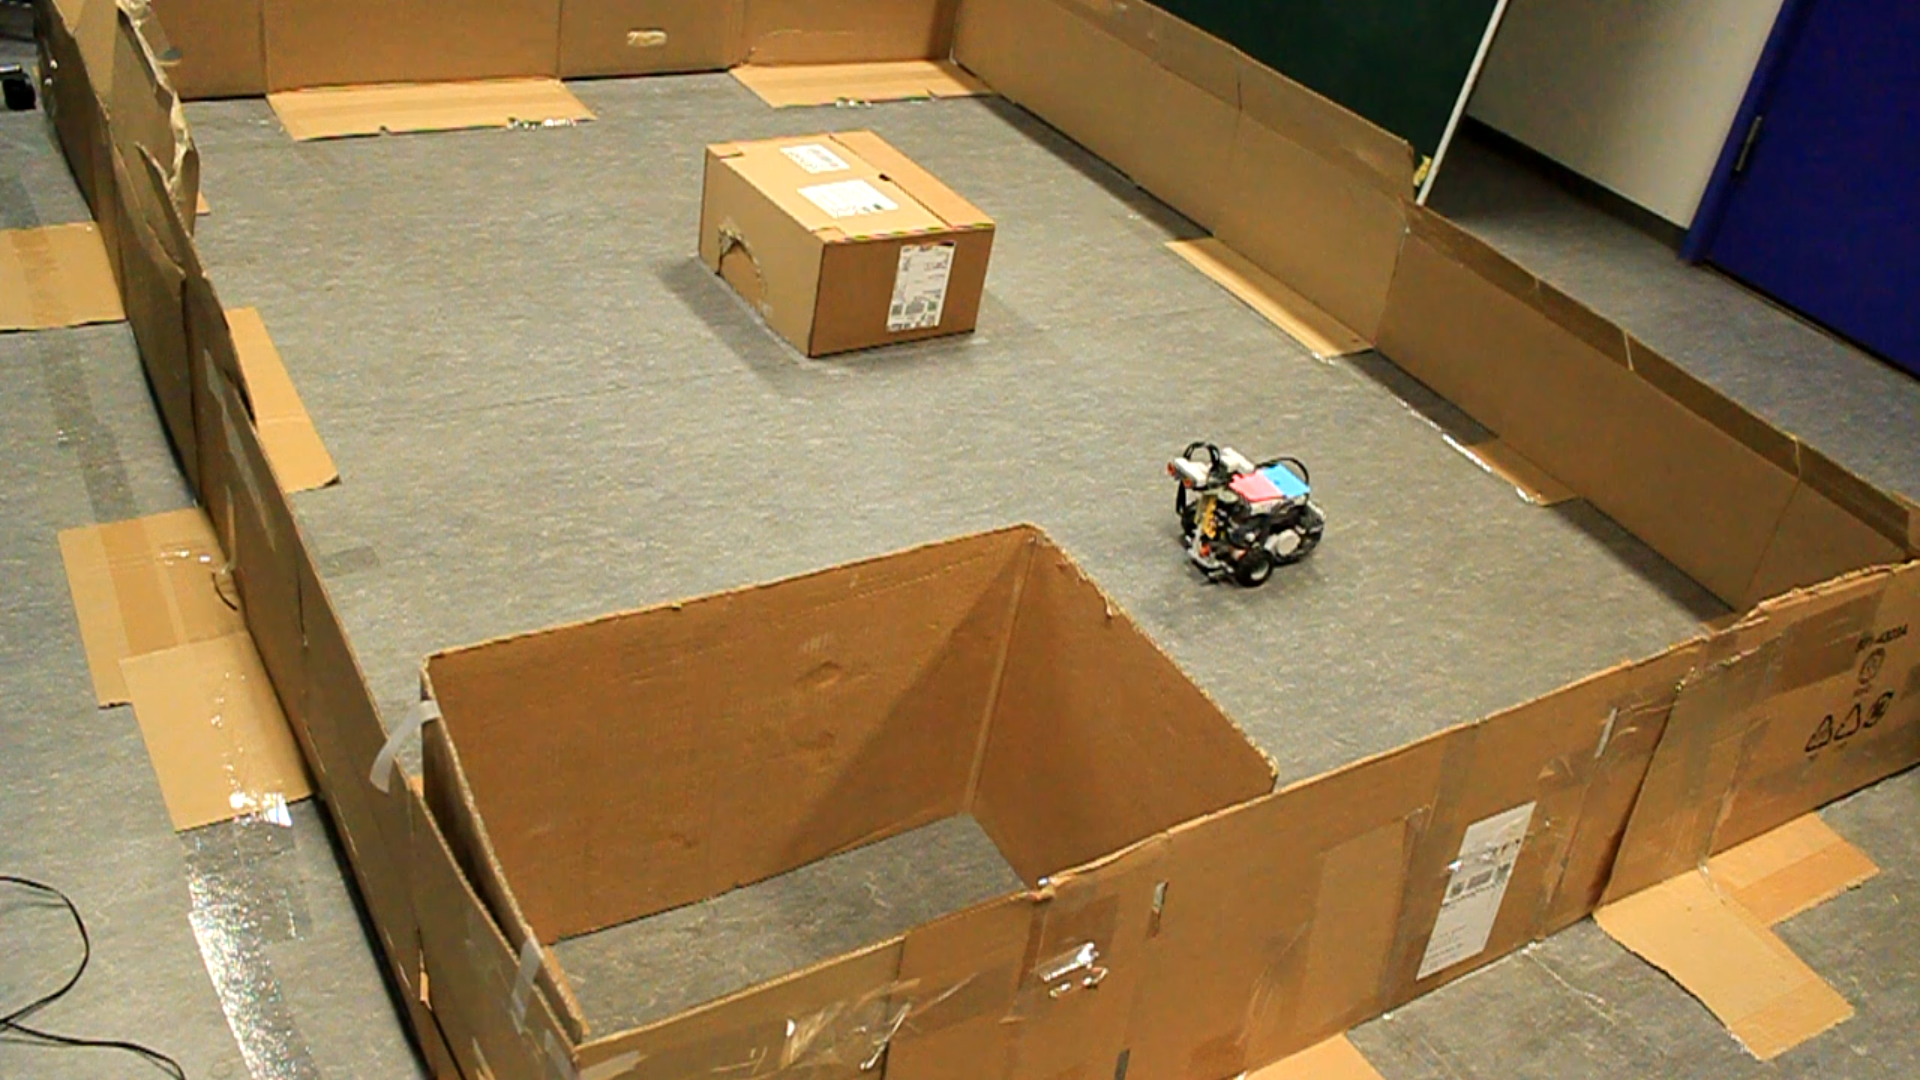
\includegraphics[width=1\textwidth]{verden/opstilling.png}
	\end{figure}
\end{frame}

\begin{frame}[fragile]{Kørselsmiljø set oppefra (Kinect)}
	\begin{figure}
		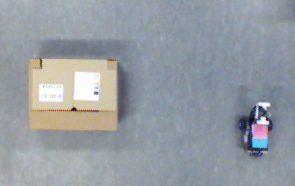
\includegraphics[width=.75\textwidth]{evaluering/emptyGrid.png}
	\end{figure}
\end{frame}

%--------------------------------------------------
%     EVALUERINGSMETODE
%--------------------------------------------------
\subsection{Evaluering af målsætning}
\begin{frame}[fragile]{Vurderingsmål}
	\linespace
	\begin{columns}
		\begin{column}{0.4\textwidth}
			\begin{itemize}
				\item Approximering af et optimalt kort for forsøgsopstillingen
			\end{itemize}
			\linespace
			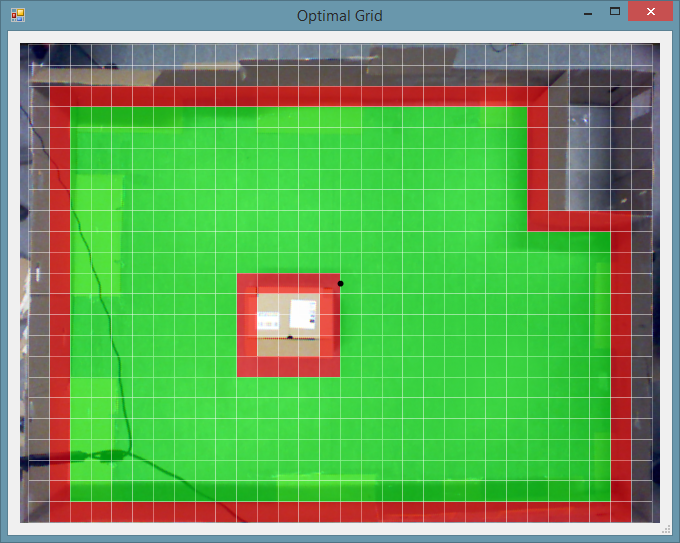
\includegraphics[width=\textwidth]{evaluering/optimalgrid.png}
		\end{column}
		
		\pause
		
		\begin{column}{0.6\textwidth}
			\begin{itemize}
				\item Vurdering af målsætning
			\end{itemize}
			\linespace
			\begin{tabular}{|l|c|c|c|}
			\hline
			& \multicolumn{3}{|c|}{Optimalt} \\
			\hline
			Test & \textbf{Optaget} & \textbf{Fri} & \textbf{Ukendt} \\ \hline
			\textbf{Optaget} & $+1$ & $-1$ & $0$ \\ \hline
			\textbf{Fri} & $-1$ & $+1$ & $0$ \\ \hline
			\textbf{Ukendt} & $-1$ & $-1$ & $0$ \\ \hline
			\end{tabular}
		\end{column}
\end{columns}
\end{frame}

% SIMPEL SENSOR MODEL
\begin{frame}[fragile]{Simpel sensormodel}
	\begin{columns}
		\begin{column}{0.5\textwidth}
			\begin{itemize}
			\item \textbf{100}/150 opdateringer
			\item \textbf{127}/555 point
			\end{itemize}
			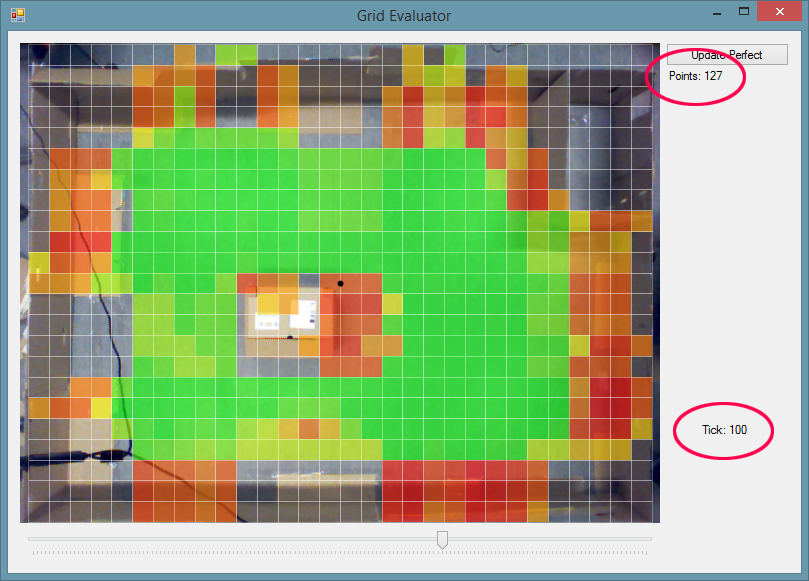
\includegraphics[width=\textwidth]{evaluering/simple3_100.png}
		\end{column}
		\begin{column}{0.5\textwidth}
			\begin{itemize}
			\item \textbf{150}/150 opdateringer
			\item \textbf{193}/555 point
			\end{itemize}
			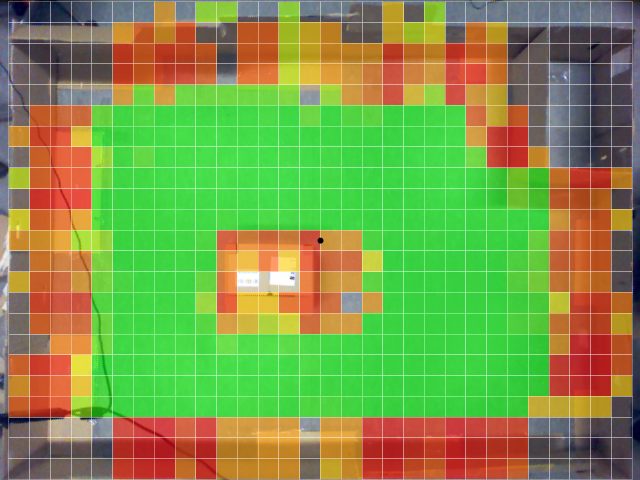
\includegraphics[width=\textwidth]{evaluering/simple3_150.png}
		\end{column}
\end{columns}
\end{frame}

% GAUSISK SENSOR MODEL
\begin{frame}[fragile]{Gausisk sensormodel}
	\begin{columns}
		\begin{column}{0.5\textwidth}
			\begin{itemize}
			\item \textbf{100}/150 opdateringer
			\item \textbf{295}/555 point
			\end{itemize}
			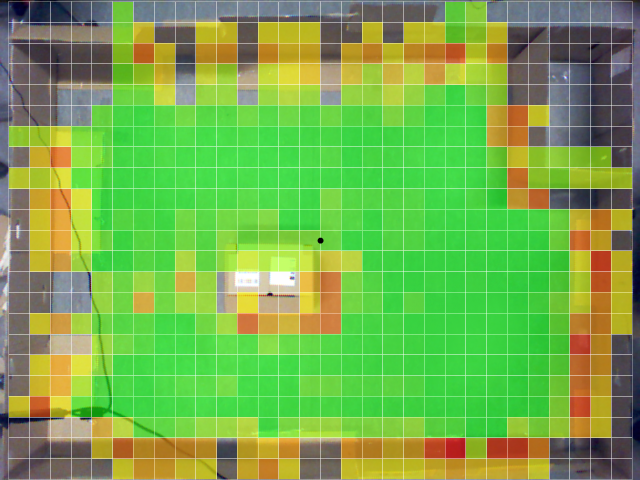
\includegraphics[width=\textwidth]{evaluering/gauss3_100.png}
		\end{column}
		\begin{column}{0.5\textwidth}
			\begin{itemize}
			\item \textbf{150}/150 opdateringer
			\item \textbf{337}/555 point
			\end{itemize}
			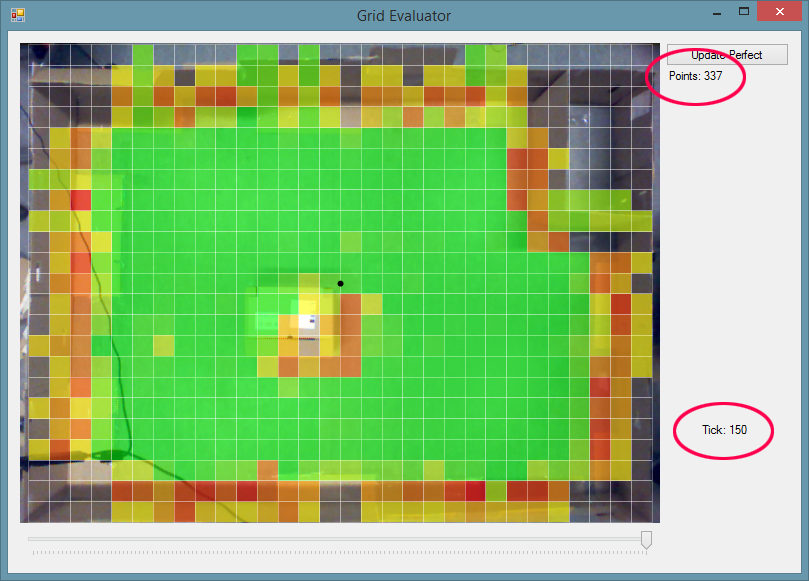
\includegraphics[width=\textwidth]{evaluering/gauss3_150.png}
		\end{column}
\end{columns}
\end{frame}

% SAMMENLIGNING AF SENSOR MODELLER
\begin{frame}[fragile]{Sammenligning af simpel- og gausisk sensormodel}
	\begin{columns}
		\begin{column}{0.5\textwidth}
			Simpel:
			\begin{itemize}
			\item \textbf{150}/150 opdateringer
			\item \textbf{193}/555 point
			\end{itemize}
			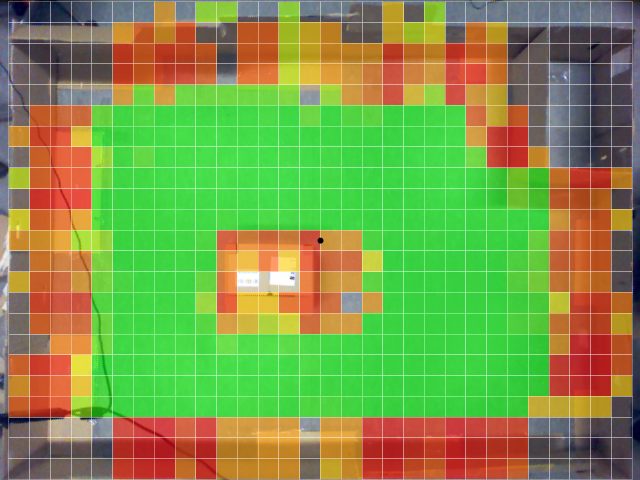
\includegraphics[width=\textwidth]{evaluering/simple3_150.png}
		\end{column}
		\begin{column}{0.5\textwidth}
			Gausisk:
			\begin{itemize}
			\item \textbf{150}/150 opdateringer
			\item \textbf{337}/555 point
			\end{itemize}
			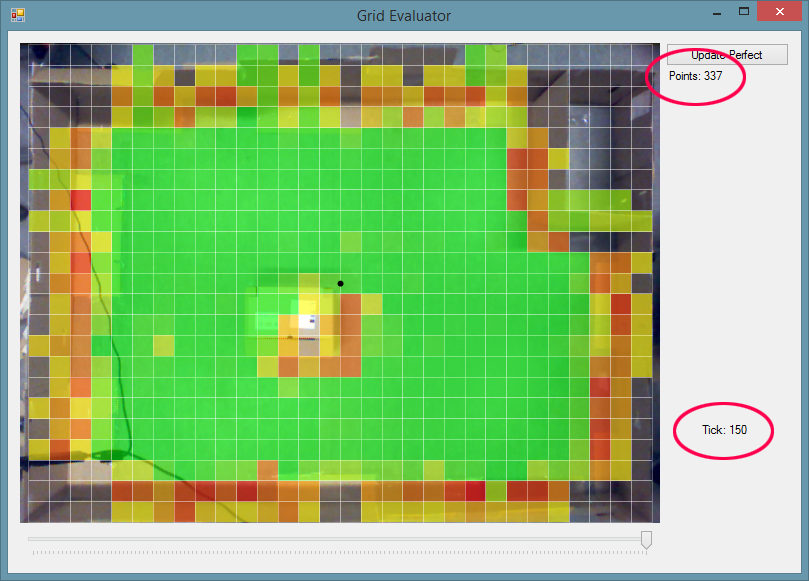
\includegraphics[width=\textwidth]{evaluering/gauss3_150.png}
		\end{column}
\end{columns}
\end{frame}